% !TeX spellcheck = en_US
\documentclass[a4paper]{report}
\usepackage[T1]{fontenc}
\usepackage[utf8]{inputenc}
\usepackage[english]{babel}
\usepackage{geometry}
\usepackage{graphicx}
\usepackage{subfig}
\usepackage{lipsum}
\geometry{a4paper,top=2.5cm,bottom=2.5cm,left=3cm,right=3cm,%
	heightrounded,bindingoffset=5mm}

\usepackage{color}
\usepackage{listings}
\usepackage{xcolor}

\colorlet{punct}{red!60!black}
\definecolor{background}{HTML}{EEEEEE}
\definecolor{delim}{RGB}{20,105,176}
\colorlet{numb}{magenta!60!black}

\lstset{ %
	language=C++,                % choose the language of the code
	basicstyle=\footnotesize,       % the size of the fonts that are used for the code
	numbers=left,                   % where to put the line-numbers
	numberstyle=\footnotesize,      % the size of the fonts that are used for the line-numbers
	stepnumber=1,                   % the step between two line-numbers. If it is 1 each line will be numbered
	numbersep=5pt,                  % how far the line-numbers are from the code
	backgroundcolor=\color{white},  % choose the background color. You must add \usepackage{color}
	showspaces=false,               % show spaces adding particular underscores
	showstringspaces=false,         % underline spaces within strings
	showtabs=false,                 % show tabs within strings adding particular underscores
	frame=single,           % adds a frame around the code
	tabsize=2,          % sets default tabsize to 2 spaces
	captionpos=b,           % sets the caption-position to bottom
	breaklines=true,        % sets automatic line breaking
	breakatwhitespace=false,    % sets if automatic breaks should only happen at whitespace
	escapeinside={\%*}{*)}          % if you want to add a comment within your code
}

\lstdefinelanguage{json}{
	basicstyle=\normalfont\ttfamily,
	numbers=left,
	numberstyle=\scriptsize,
	stepnumber=1,
	numbersep=8pt,
	showstringspaces=false,
	breaklines=true,
	frame=lines,
	backgroundcolor=\color{background},
	literate=
	*{:}{{{\color{punct}{:}}}}{1}
	{,}{{{\color{punct}{,}}}}{1}
	{\{}{{{\color{delim}{\{}}}}{1}
	{\}}{{{\color{delim}{\}}}}}{1}
	{[}{{{\color{delim}{[}}}}{1}
	{]}{{{\color{delim}{]}}}}{1},
}

%{0}{{{\color{numb}0}}}{1}
%{1}{{{\color{numb}1}}}{1}
%{2}{{{\color{numb}2}}}{1}
%{3}{{{\color{numb}3}}}{1}
%{4}{{{\color{numb}4}}}{1}
%{5}{{{\color{numb}5}}}{1}
%{6}{{{\color{numb}6}}}{1}
%{7}{{{\color{numb}7}}}{1}
%{8}{{{\color{numb}8}}}{1}
%{9}{{{\color{numb}9}}}{1}

\newcommand{\HRule}{\rule{\linewidth}{0.5mm}}

\begin{document}
\begin{titlepage}
	\begin{center}
		
		% Top 
		
\includegraphics[width=0.45\textwidth]{img/unipi.png}~\\[2.5cm]
		
		
		% Title
		\HRule \\[0.4cm]
		{ \LARGE 
			\textbf{JustRecipe}\\[0.4cm]
			\emph{Group Project for Large Scale and Multi-Strutured Databases}\\[0.4cm]
		}
		\HRule \\[1.5cm]
		
		
		
		% Author
		{ \large
			Francesco Campilongo \\[0.1cm]
			Daniele Cioffo \\[0.1cm]
			Francesco Iemma \\[0.1cm]
		}
		
		\vfill

		%\textsc{\large Department of Electrical Engineering,\\Computer Engineering \& Informatics}\\[0.4cm]
		
		
		% Bottom
		{\large Academic Year 2020/21}
		
	\end{center}
\end{titlepage}


\tableofcontents

\chapter*{Introduction}

\chapter{Dataset}
In this first chapter of this document we will talk about searching for the initial dataset.

\noindent As specified in the project documentation, the dataset had to be at least 50MB large, and this quantity could not be generated directly within the application. So we did an initial search, finding two datasets, which were generated by their authors by performing the scraping on the sites \emph{www.FoodNetwork.com} and \emph{www.Epicurios.com}. The second dataset was more complete (more nutritional values), so it was used as the main dataset. The other dataset was used to complement the other, reaching a total of  67.8 MB, with 45349 recipes.

\noindent To correctly extract the data present in the two datasets we wrote a program in Java, called \emph{RecipeReade}r, thanks to which we adapted the two different formats and removed the duplicates (recipes with the same title that were present in both datasets).
To implement this program we used the GSon library and the Jackson library.

\noindent The variety property is ensured by using two different sources. The velocity / variability properties are ensured because comments and recipes are eliminated and added inside the application, indeed this data may lose importance after a certain time interval since new data quickly arrives.

\chapter{Design}
\section{Introduction To The Application}
The topic of cuisine is extensively widespread in our society. In fact we can think at the success achieved by tv shows related to cooking in the last years and also at the fact that a lot of chefs are becoming superstars.
Then there is another important factor: the coronavirus outbreak.

\noindent With the coronavirus outbreak a lot of people became cuisine lovers, in fact at the first moments of the pandemia several ingredients as flour and yeast were very hard to find, because people were confined in their home and so they had more free time.

\noindent But this topic is not a recente one. The first recipe book dates back to eigth century B.C. and it is the so-called \emph{Eraclio} (by the name of the city in which he was found). Then also an important latin writer, Apicio, wrote one of the most important recipe books of the roman era: \emph{De Re Coquinaria} which dates back to the first century B.C..
 
\noindent So the topic of cuisine is inherent to human nature, because the necessity of eating is a basic need.
Furthermore, everyone has experimented the infamous question: “What will I eat this evening?”. JustRecipe has the aim of answer to this question, it has the aim of helping university student or workers to retrieve and to do fast and simple recipes.

\noindent So this application is basically a recipe book but it is also more than this.

\noindent JustRecipe is also a social network which allow people to enjoy, to ex-change ideas about cooking, to feel less lonely in this hard period.

\section{Requirements}
\subsection{Main Actors}
The main actors of the application are four:
\begin{itemize}
	\item Unregistered User
	
	\noindent He is the user which open the application for the first time, in order to access he must sign-up.
	
	\item User
	
	\noindent He is the normal user (the registered one).
	
	\item Moderator
	
	\noindent He is in charge of controlling the comments and eventually delete the ones which contain abuses.
	
	\item Administrator
	
	\noindent He is the most powerful actor, he can delete users and recipes and he is also in charge of elect moderators
\end{itemize}

\noindent Each actor can do all the features of the previous ones in the list.

\subsection{Functional Requirements}
\subsubsection{Features offered to the Unregistered User}
\begin{itemize}
	\item  Registration
	
	\noindent In order to access the application an user must sign-up. Otherwise he is not allowed to access and to use all the functionalities.
\end{itemize}
\subsubsection{Features offered to the Registered User}
\begin{itemize}
	\item Login/Logout
	
	\noindent The only way to access the application, as we said previously, is to sign-up and login. At the end the user can logout and close the session.
	
	\item Search a recipe
	
	\noindent It's possible to search a recipe searching for the title and for categories.
	
	\item Browse suggested recipes
	
	\noindent The suggestions will be offered in a proper section, they are done considering the relationships between the user logged, the users followed by the user logged and so on so forth.
	
	\item Browse recipes of following users
	
	\noindent In a proper section (i.e. the Homepage) the user can browse the recipes of the following user. Indeed he can see only a snapshot of the recipes. If he wants a more in-depth view, he can click on it and see the recipe page in which he is able to see all the recipe details. 
	
	\item Add a recipe
	
	\noindent The user can insert a new recipe.
	
	\item Edit own recipes
	
	\noindent The user can edit the recipes previously added by himself.
	
	\item Comment recipes
	
	\noindent
	Every user can make a comment about recipes
	
	\item Follow another user
	
	\noindent The most important feature of each social network: the users can follow each others. 
	
	
	\item Like a recipe
	
	\noindent In order to evaluate a recipe each user can like its.
\end{itemize}

\subsubsection{Features offered to the Moderator}
\begin{itemize}
	\item Delete comments
	
	\noindent The moderator is in charge of delete comments which contain racist abuse, crude terms and so on so forth.
\end{itemize}

\subsubsection{Features offered to the Administrator}
\begin{itemize}
	\item Delete users
	
	\noindent The admin can delete the users which don't respect the application guidelines.
	
	\item Delete recipes
	
	\noindent The admin can delete recipes not correctly inserted
	
	\item Elect moderators
	
	\noindent In order to handle better the application, the admin can elect some users as moderators.
\end{itemize}
\subsection{Non-Functional Requirements}

\subsection{Actors and Use Cases}
The use case diagram of the application is described in the figure 2.1

\begin{figure}[htpb]
	\centering
	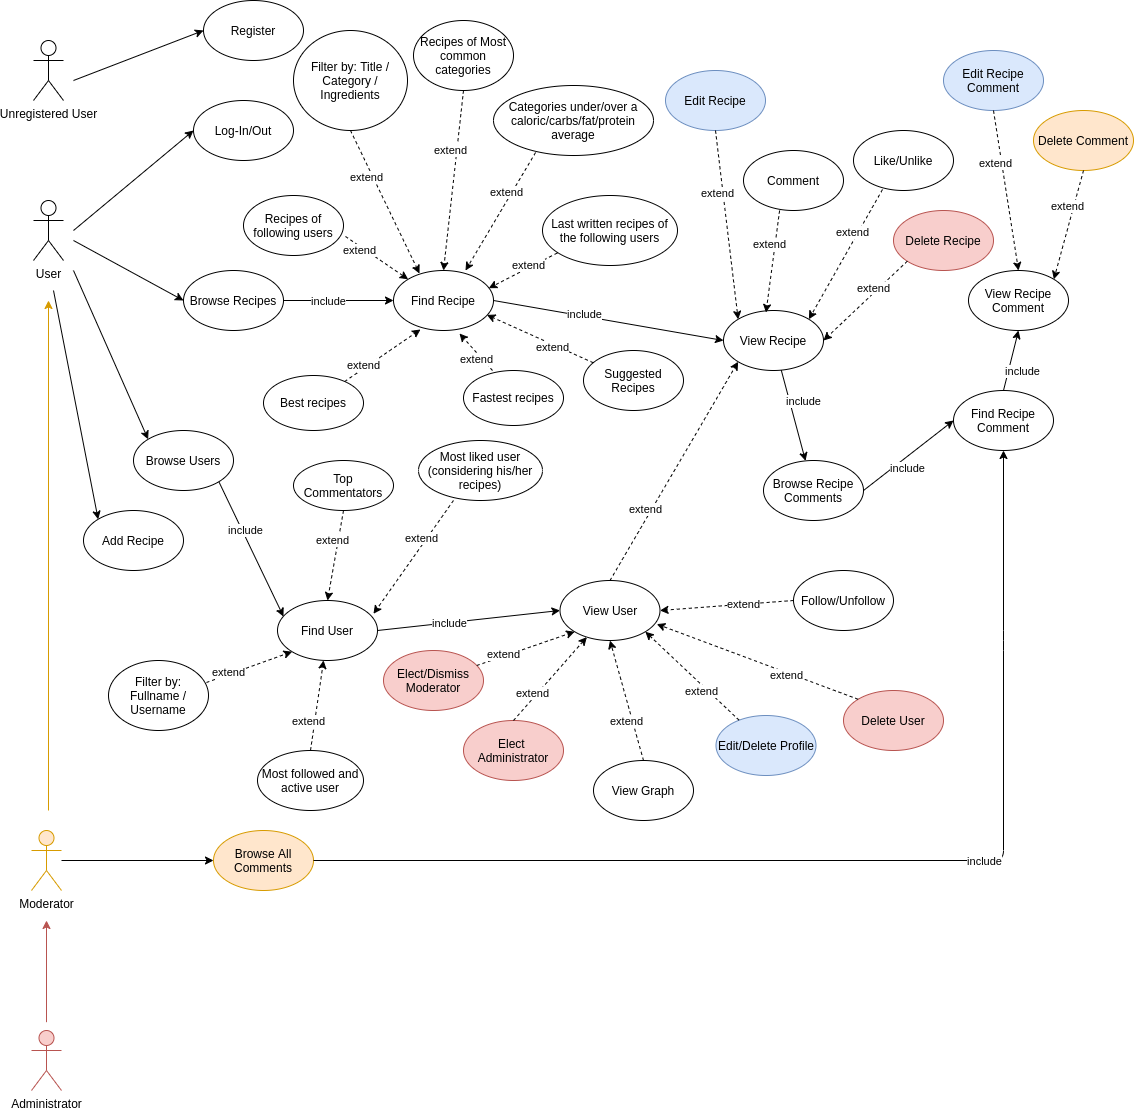
\includegraphics[scale=0.42]{img/UseCaseDiagram.png}
	\caption{Use Case Diagram}
\end{figure}
Some observations on the diagram are necessary:
\begin{itemize}
	\item The circles in \underline{blue} are the ones which described actions available only for the owner of the object on which the actions are applied.
	
	\noindent So, in detail, this means that a \textbf{User} can edit/delete a profile if and only if he owns this profile. Then he can edit a recipe and/or a comment if and only if he adds that recipe or that comment.
	
	\item When we are seeing the recipe detail we can go on the user that have been added that recipe. So the extend relation between \emph{View Recipe} and \emph{View User} means this.
	
	\item The action \emph{Browse Recipes of following users} is available only if the \textbf{User} follows at least one user. Otherwise he can start to follow users and only after this he can see suggested recipes (\emph{Browse Suggested Recipes}). In this case, due to the fact that the user follows nobody, he will see the most famous recipes in general because it's impossible to suggest specific recipes due to the fact that he has no following and no likes or comments. 
	
	\item The actions in \underline{red} are the ones that can be performed only by the \textbf{Administrator}
	
	\item The actions in \underline{orange} are the ones that can be performed only by the \textbf{Moderators}
\end{itemize}


\section{UML Class Diagram}
Let analyze the UML Class Diagram. There are three main entities: User, Comment, Recipe.

\noindent It's important to point out that the \textbf{User} of the Use Case Diagram is here the so-called \emph{Registered User} and the \emph{User} of this diagram is the generic user. Then we undeline the fact that, in order to represent the three actors of the use case diagram, a generalization is needed.
 
\begin{figure}[htpb]
	\centering
	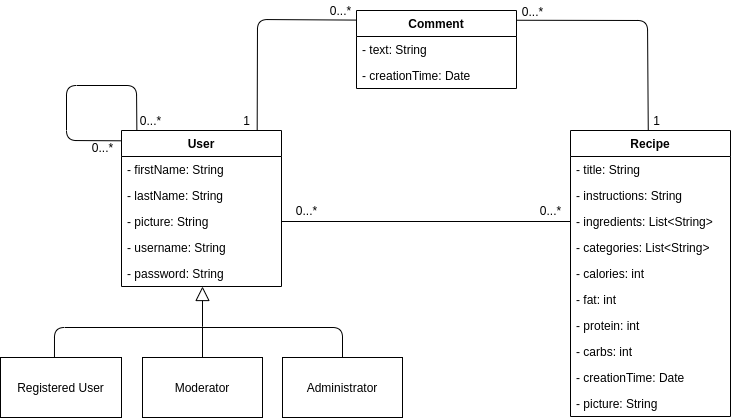
\includegraphics[scale=0.5]{img/ClassDiagram_generaliz.png}
	\caption{UML Analysis Classes Diagram with generalization unsolved}
\end{figure}

\noindent Observing the figure 2.2 it's possible to understand that we can resolve the generalization putting an attribute in the entity \emph{User}. It is an integer and we call it \emph{role}: if it's a \emph{Normal User} role is 0; if \emph{Moderator} then 1; if \emph{Administrator} then 2.

\begin{figure}[htpb]
	\centering
	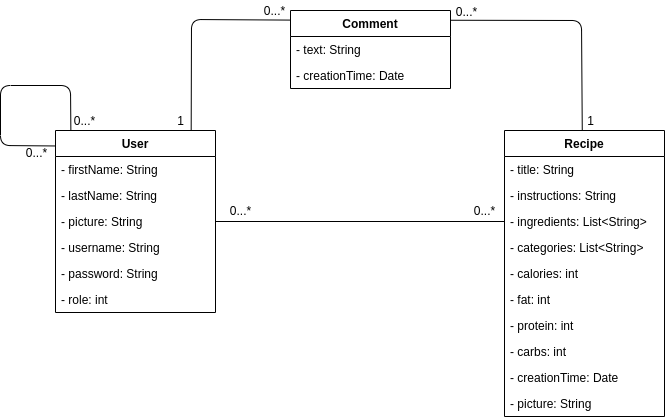
\includegraphics[scale=0.5]{img/ClassDiagram.png}
	\caption{UML Analysis Classes Diagram}
\end{figure}

\section{Data Model}

\subsection{DocumentDB}
\lstset{ language=json}
\begin{lstlisting}
{
	"_id":
			{"$oid": "5fdb5fd86796ee4e73ef5b84"},
	"title": 
			"Lentil, Apple, and Turkey Wrap ",
	"instructions": 
			"1. Place the stock, lentils, celery, carrot, thyme, and
			salt in a medium saucepan and bring to a boil. Reduce heat
			to low and simmer until the lentils are tender, about 30
			minutes, depending on the lentils. (If they begin to
			dry out, add water as needed)..." ,
	"ingredients":
			["4 cups low-sodium vegetable or chicken stock", "1 cup dried brown lentils", ...],
	"categories":
			["Sandwich", "Bean", "Fruit", "Tomato", "turkey", ...],
	"calories":
			426,
	"fat":
			7,
	"protein":
			30,
	"carbs":
			20,
	"creationTime":
			{
				"$date": "2020-12-17T13:40:40.658Z"
			},
	"authorUsername":
			"oscar.evans",
	"picture":
			"https://assets.epicurious.com/photos/551b0595e7851a541a30b23f/master/pass/239173_lentil-apple-and-turkey-wrap_6x4.jpg",
	"comments":
			[
				{
					"authorUsername": "oliver.smith",
					"text": "Very good!!!",
					"creationTime":
					{
						"$date": "2020-12-17T13:50:40.658Z"
					}
				},
				{
					"authorUsername": "jessica.evans",
					"text": "Fantastic",
					"creationTime":
					{
						"$date": "2020-12-17T13:52:40.658Z"
					}
				},....
			]
}
\end{lstlisting}  
\subsection{GraphDB}
\section{Distributed Database Design}
\subsection{Replicas}
\subsection{Sharding}
\section{Software Architecture}


\chapter{Implementation and Test}
\section{Main Modules}
\section{Main Packages and Classes}
\section{Most Relevant Queries}
\subsection{MongoDB}
\subsection{Neo4J}
\section{Unit Test}
\section{Tests and Statistical Analysis}

\chapter{User Manual}
\end{document}
